\chapter{Requisitos y diseño}
\label{cap:introduccion}


%\begin{resumen}

%Resumen: En este capítulo se explicarán los prototipos de la aplicación realizados por Alfonso y Jorge (Sección \ref{cap4:diseñoapp}). Después se analizarán ambos prototipos y se definirán los requisitos (Sección \ref{cap4:requisitosapp}) que deberían incluirse en el desarrollo PictUp!.
	
%\end{resumen}

\label{cap1:sec:Motivacion}


\section{Introducción}
De ahora en adelante se referirá a la aplicación como PictUp!. El propósito de la aplicación PictUp! es solventar problemas encontrados en otras aplicaciones similares y combinar las herramientas necesarias para facilitar la creación de materiales pictográficos. Para ello, se han estudiado las características de las distintas aplicaciones vistas en la Sección \ref{cap2:tablacomparativa}. De esta manera, se han seleccionado las funcionalidades imprescindibles para crear un tablero pictográfico y otras atendiendo a las necesidades demandadas por los usuarios. Así se ha podido confeccionar una lista de requisitos iniciales de la aplicación y el motivo de su interés. A continuación, se expondrán las caracterísiticas que debería reunir PictUp!: 


\begin{itemize}
	\item \textbf{Crear tableros con facilidad y precisión}: los pictogramas que se coloquen en el tablero deben de poder alinearse sencillamente. 
	\item \textbf{Utilizar fotografías como material}: algunos usuarios quieren complementar los tableros con imágenes propias que pueden ser más familiares a la persona que se beneficie del tablero. 
	\item \textbf{Agilizar el proceso de búsqueda de pictogramas que sean usados de manera recurrente}: al crear material de manera recurrente puede ser útil contar con los pictogramas más usados para no repetir la misma búsqueda repetidamente. 
	\item \textbf{Añadir interacción a los tableros}: la mayoría de las aplicaciones estudiadas son estáticas, es decir, no permiten una interacción adicional al usuario con el tablero. Algunas aplicaciones aprovechan dicho potencial como Piktoplus (Sección \ref{cap2:pkplus}) mediante los subtableros emergentes o Jocomunico (Sección \ref{cap2:jocomunico}) que permite reproducir la pronunciación del texto asociado a un pictograma.
	
\end{itemize}






\section{Diseño de la aplicación}
\label{cap4:diseñoapp}
Después de probar distintas tecnologías y estudiar la situación actual de los tableros pictográficos, se procedió a bocetar la idea de la aplicación y el formato de la interfaz. Al ser dos integrantes en el proyecto, se realizaron dos bocetos diferentes, a partir de los cuales se concretaron los primeros requisitos y asentaron las bases del proyecto.


\subsection{Prototipo realizado por Alfonso}
\label{cap4:sec:alfonso}
Teniendo en cuenta los requisitos de los usuarios, las aplicaciones existentes y el trabajo futuro de trabajos similares, empezamos a bocetar una primera idea del proyecto.


En la Figura \ref{fig:loginalfonso} podemos ver el boceto de la pantalla de  inicio, la cual estaría compuesta por cuatro secciones bien diferenciadas. \textit{Creación de tablero libre} serviría para crear un tablero donde se pueden colocar pictogramas, texto o figuras. \textit{Creación de actividad} añadiría interacción a los tableros mediante la sucesión de los mismos. Más tarde profundizaremos en esas dos secciones.

% TODO: \usepackage{graphicx} required
\begin{figure}[h!]
	\centering
	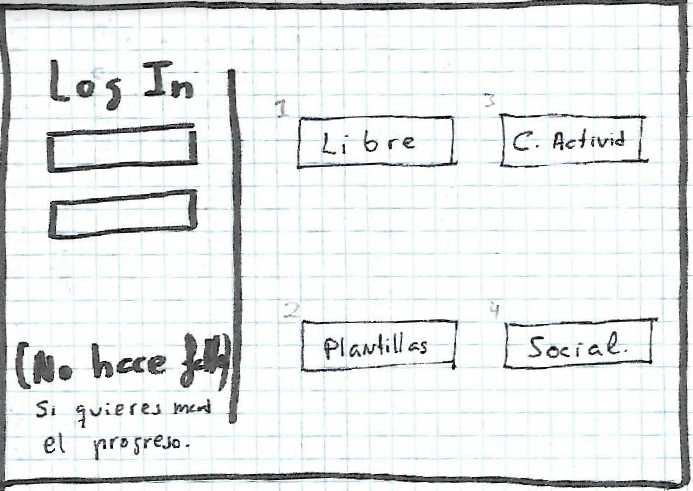
\includegraphics[width=0.7\linewidth]{Imagenes/Bitmap/logInAlfonso}
	\caption{Boceto de pantalla inicial}
	\label{fig:loginalfonso}
\end{figure}

Las \textit{Plantillas} permitirían crear un tablero mediante el uso de una plantilla que cuenta con espacios donde colocar pictogramas. Las plantillas facilitan la creación del material que sigue una misma estructura, pero con contenido diferente. Un ejemplo de ello es la creación de un horario, donde pueden haber decenas de huecos a rellenar y se estructuran generalmente de la misma manera. Al tener una plantilla, el usuario se puede despreocupar de que los elementos queden bien centrados o añadir los días de la semana. En la Figura \ref{fig:inicioalfonso} podemos ver un ejemplo de algunas ideas de plantillas disponibles. 
La sección de \textit{Social} tendría la función de compartir tableros, actividades y plantillas con la comunidad de usuarios. Por último, existe un inicio de sesión opcional para mantener el progreso entre dispositivos.

% TODO: \usepackage{graphicx} required
\begin{figure}[h!]
	\centering
	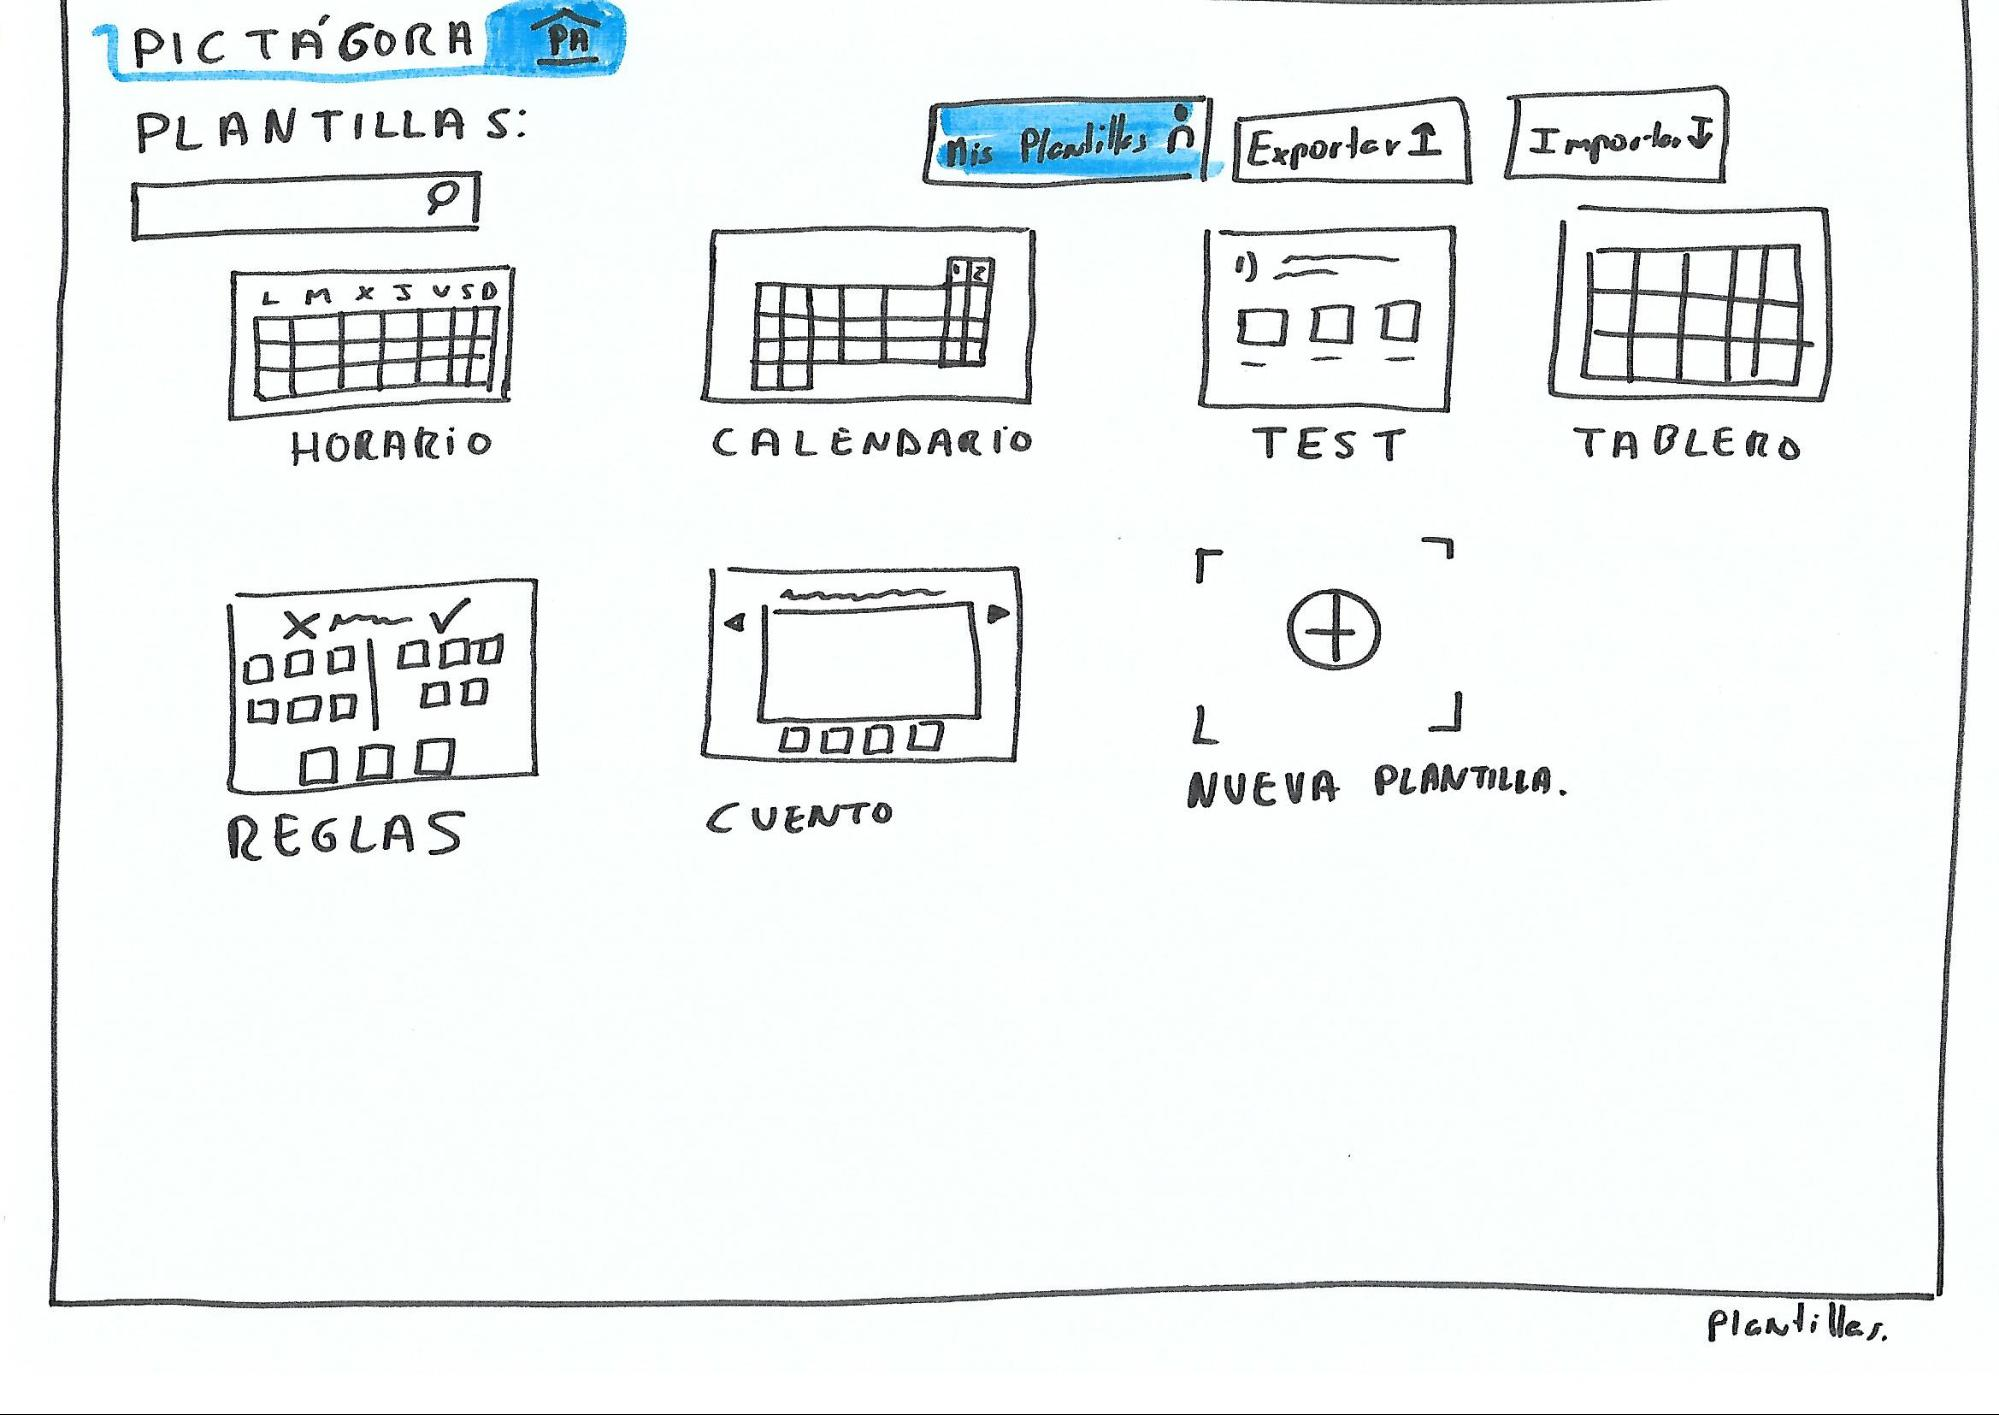
\includegraphics[width=0.7\linewidth]{Imagenes/Bitmap/inicioAlfonso}
	\caption{Boceto pantalla de plantillas}
	\label{fig:inicioalfonso}
\end{figure}


 Si profundizamos en la \textit{Creación de un tablero libre} en la Figura \ref{fig:dibujolibrealfon}, podemos ver los componentes que se pueden colocar sobre el tablero. Éstos son los pictogramas, texto, figuras como flechas o rectángulos y la posibilidad de subir imágenes. También comenzamos a plantear la idea de almacenar colecciones de pictogramas, que almacenan distintos conjuntos de pictogramas que el usuario agrupa según su criterio. Por ejemplo, si un profesor tiene que crear varios tableros respecto a un tema, como “Animales de la granja”, puede ser útil tener una colección con los pictogramas de gallina, cabra, oveja, etc, agilizando el proceso de creación.

% TODO: \usepackage{graphicx} required
\begin{figure}[h!]
	\centering
	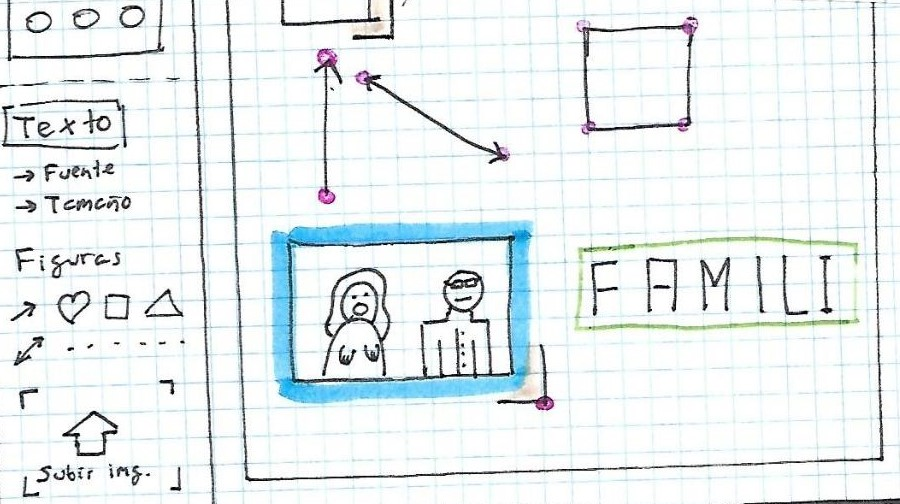
\includegraphics[width=0.7\linewidth]{Imagenes/Bitmap/DibujoLibreAlfon}
	\caption{Boceto pantalla de edición de tableros }
	\label{fig:dibujolibrealfon}
\end{figure}

El apartado de \textit{Creación de actividad} no deja de ser una extensión de creación libre pero con más  componentes que permiten interacción con el usuario para crear distintos tipos de actividad. Estos componentes, que a partir de ahora denominaremos componentes interactivos, son:

\begin{itemize}
	
	\item \textbf{Cajón de pictgramas y espacio picto}: se trata de dos componentes que van ligados entre sí. En primer lugar está el \textit{cajón de picto}, que es un espacio al margen del tablero donde aparecen un conjunto de pictogramas, como se puede ver en la Figura \ref{fig:componentecajon}. Los elementos que aparecen en el cajón pueden  ser desplazados a un \textit{espacio picto}. Este componente es un hueco inicialmente vacío donde puede ser colocado un pictograma como se puede ver también en la Figura \ref{fig:componentecajon}. Ambos componentes son configurables, lo que permite establecer los pictogramas que aparecen en el \textit{cajón de pictogramas}, y los pictogramas que acepta el \textit{espacio picto}. Ambos elementos se beneficiarían de las colecciones, pues son conjuntos de pictogramas establecidos por el usuario.
	
	% TODO: \usepackage{graphicx} required
	\begin{figure}[h!]
		\centering
		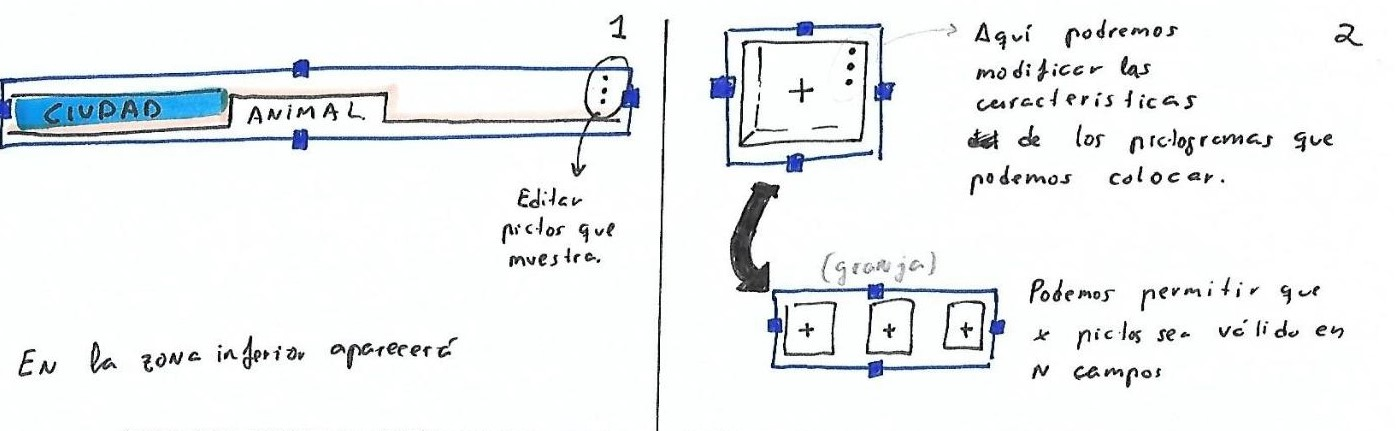
\includegraphics[width=0.7\linewidth]{Imagenes/Bitmap/componenteCajon}
		\caption{Boceto de las componentes canjón de picto y espacio picto.}
		\label{fig:componentecajon}
	\end{figure}
	
	
	Por ejemplo, un cajón de pictogramas podría tener asignado varias colecciones de pictogramas para que aparezcan mezclados. Asimismo, en el \textit{espacio picto} podría ser configurado para únicamente aceptar pictogramas de una de las colecciones o un pictograma concreto. De esta manera podría ser construido con facilidad un ejercicio donde el usuario que interactúe con el tablero pueda arrastrar distintos pictogramas del cajón de pictos a un espacio picto. En la Figura \ref{fig:cajonpictosgranja} se ve el \textit{cajón de pictos} mostrando pictogramas que representan animales de la granja y la selva, junto a unos \textit{espacio pictos} donde colocar los pictos de cada tipo.  El objetivo es dar la máxima flexibilidad al usuario que cree una actividad.
	
	
	% TODO: \usepackage{graphicx} required
	\begin{figure}[h!]
		\centering
		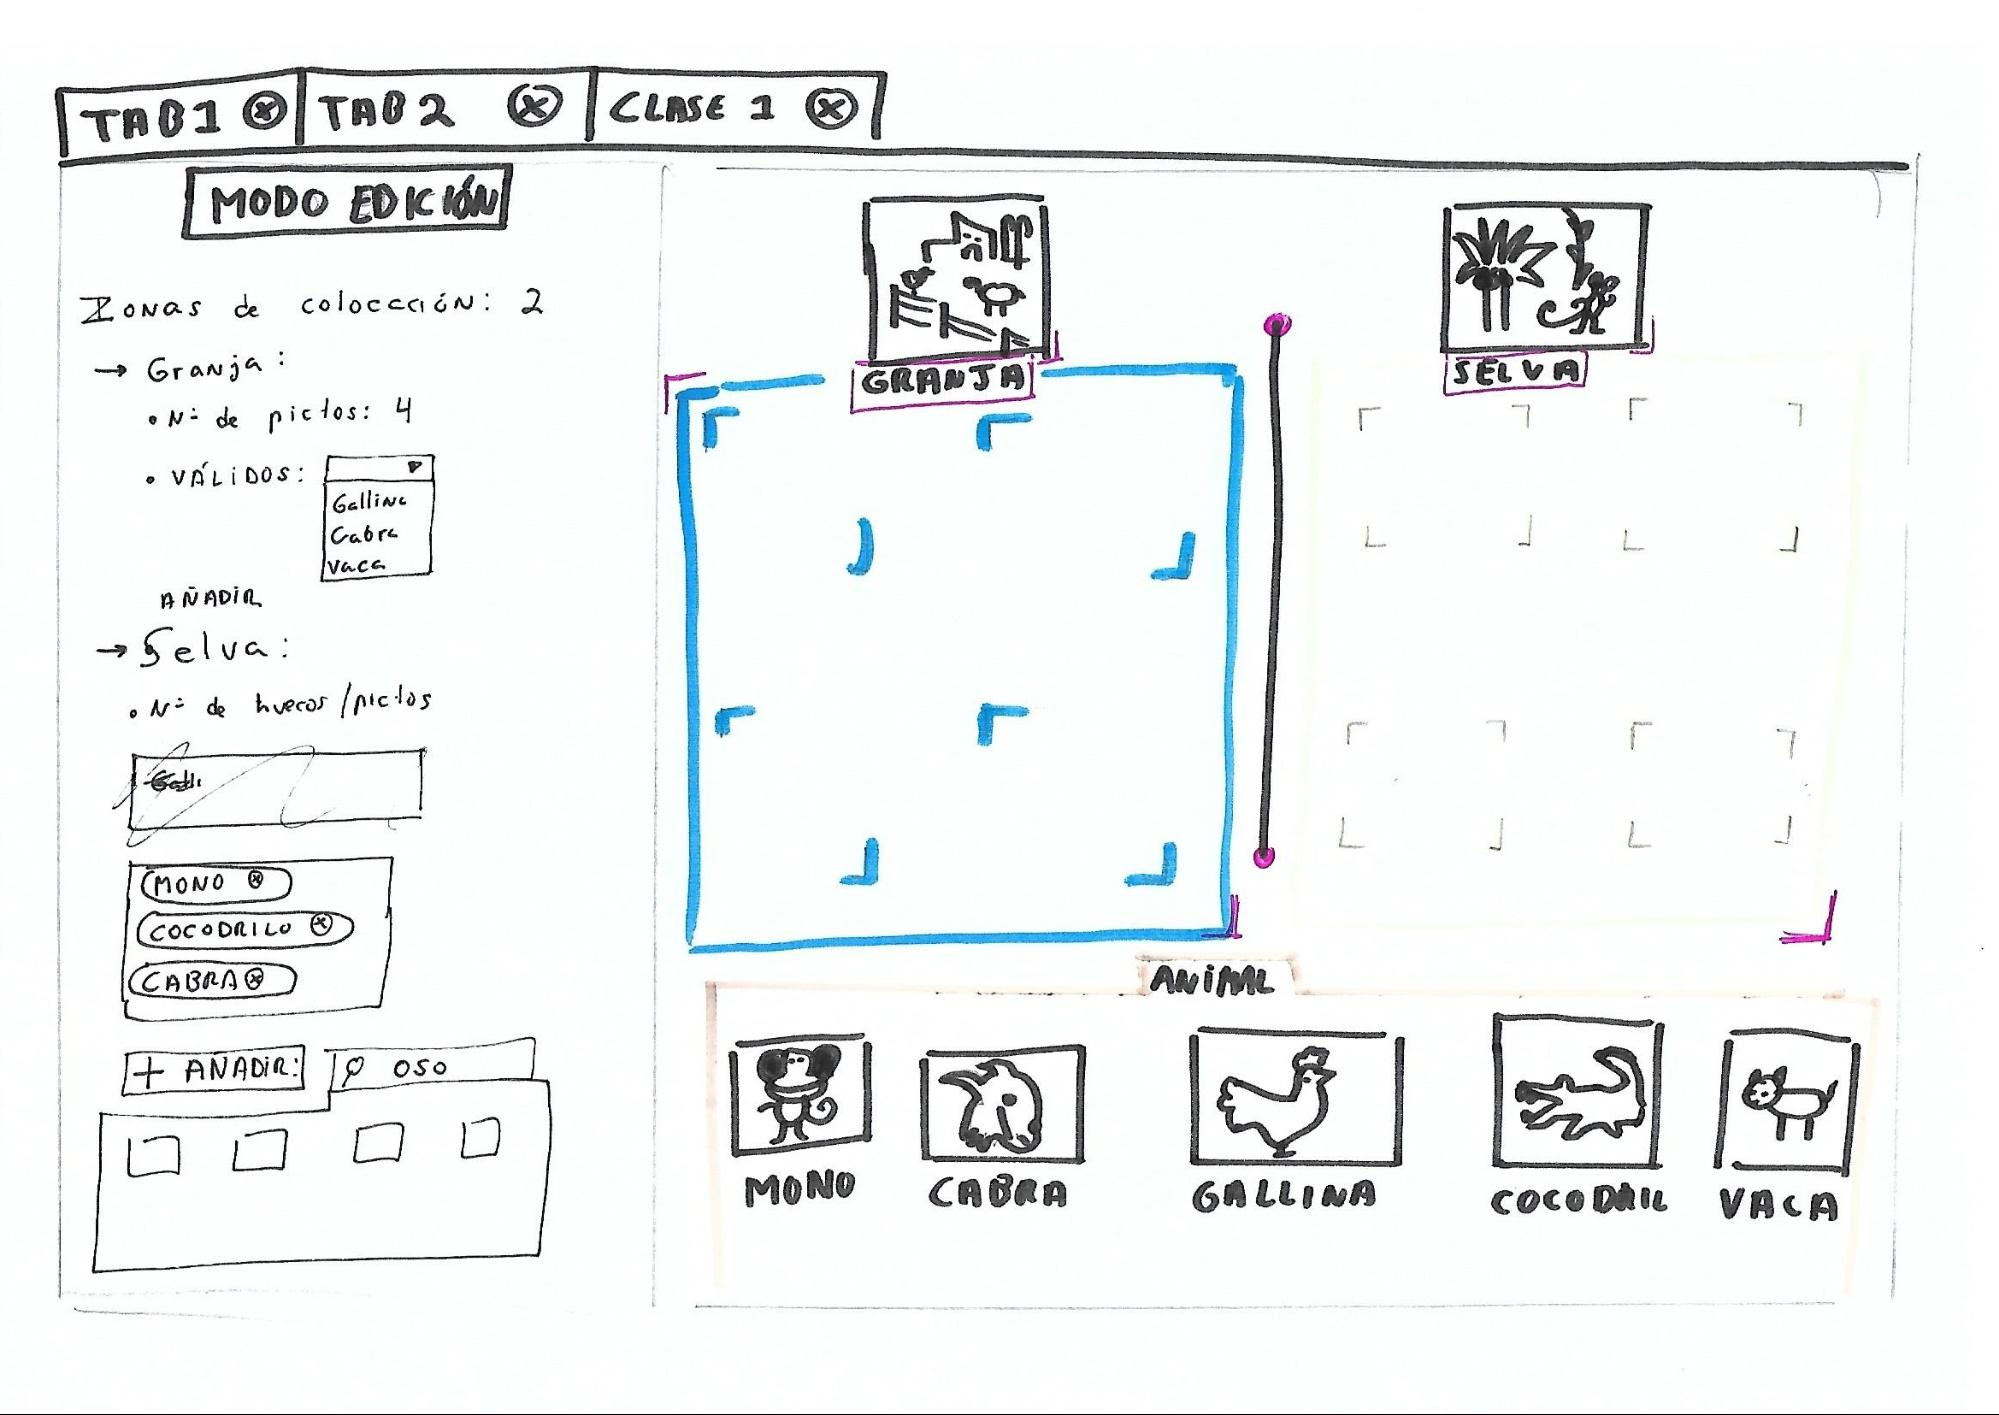
\includegraphics[width=0.9\linewidth]{Imagenes/Bitmap/cajonPictosGranja}
		\caption{Boceto de actividad con cajón de pictos y hueco picto}
		\label{fig:cajonpictosgranja}
	\end{figure}

	\item \textbf{Subtablero}: el componente subtablero permite desplegar un tablero de pictogramas. Los pictogramas que componen dicho tablero pueden venir dados por una colección de pictogramas creada por el usuario o indicarse en el propio componente. Su finalidad es la de añadir más pictogramas en el mismo espacio y agilizar la comunicación. La idea ha sido rescatada de Piktoplus (Sección \ref{cap2:pkplus}) que también permitía crear subtableros.
	
	\item \textbf{Enlace}: permite ligar dos pictogramas diferentes. Está compuesto por dos “piezas” las cuales se asignan a dos pictogramas para ser enlazados. Su finalidad es la de crear actividades como “hacer parejas”.
	
	En la Figura \ref{fig:componenteenla} podemos ver el ejemplo del pictograma hueso y perro, a los cuales se les asignan la misma pieza identificada por un símbolo de pica con fondo verde. El motivo por el que  las piezas tienen una forma y color asociado facilita al usuario que cree la actividad identificar las piezas ya  ligadas. El usuario final al pulsar sobre los pictos permitirá hacer parejas y completar la actividad.
	
	% TODO: \usepackage{graphicx} required
	\begin{figure}[h!]
		\centering
		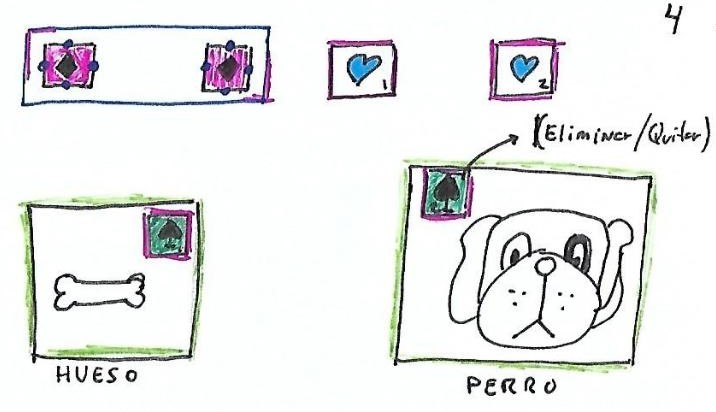
\includegraphics[width=0.7\linewidth]{Imagenes/Bitmap/componenteEnla}
		\caption{Boceto de las piezas que enlazan dos pictogramas al compartir la misma figura}
		\label{fig:componenteenla}
	\end{figure}

	
\end{itemize}

Con todos los tableros creados también es posible crear una actividad de mayor tamaño mediante la secuenciación de tableros. Se podría pasar de uno a las siguientes escenas mediante flechas, como se puede ver en la Figura \ref{fig:cuento}, que está compuesta por una fotografía y algunos pictogramas que la describen. Pero también se podrían intercalar estos tableros con otros que aporten interacción. Por ejemplo podría añadirse un test mediante el cajón de pictos para comprobar si se está comprendiendo la lectura.

% TODO: \usepackage{graphicx} required
\begin{figure}[h!]
	\centering
	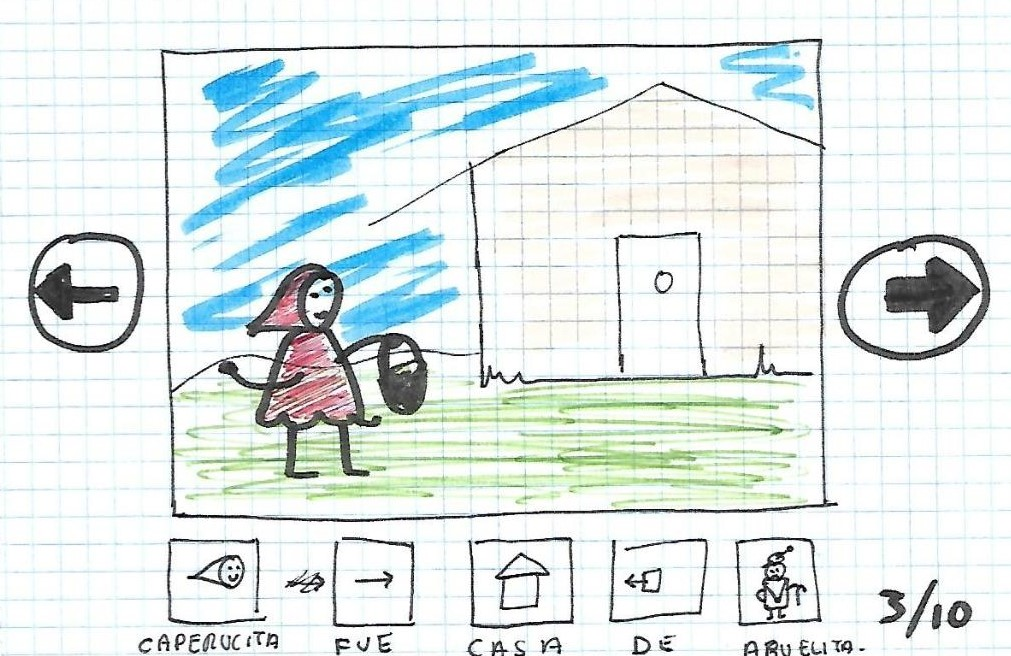
\includegraphics[width=0.7\linewidth]{Imagenes/Bitmap/Cuento}
	\caption{Boceto de una escena de un cuanto, con pictogramas en la zona inferior y botones en los laterales para pasar o retroceder la escena o tablero}
	\label{fig:cuento}
\end{figure}


En la Figura \ref{fig:presentaciontableros} podemos ver cómo se compondrían este tipo de actividades, que resulta muy familiar a la construcción de una presentación de diapositivas.  

% TODO: \usepackage{graphicx} required
\begin{figure}[h!]
	\centering
	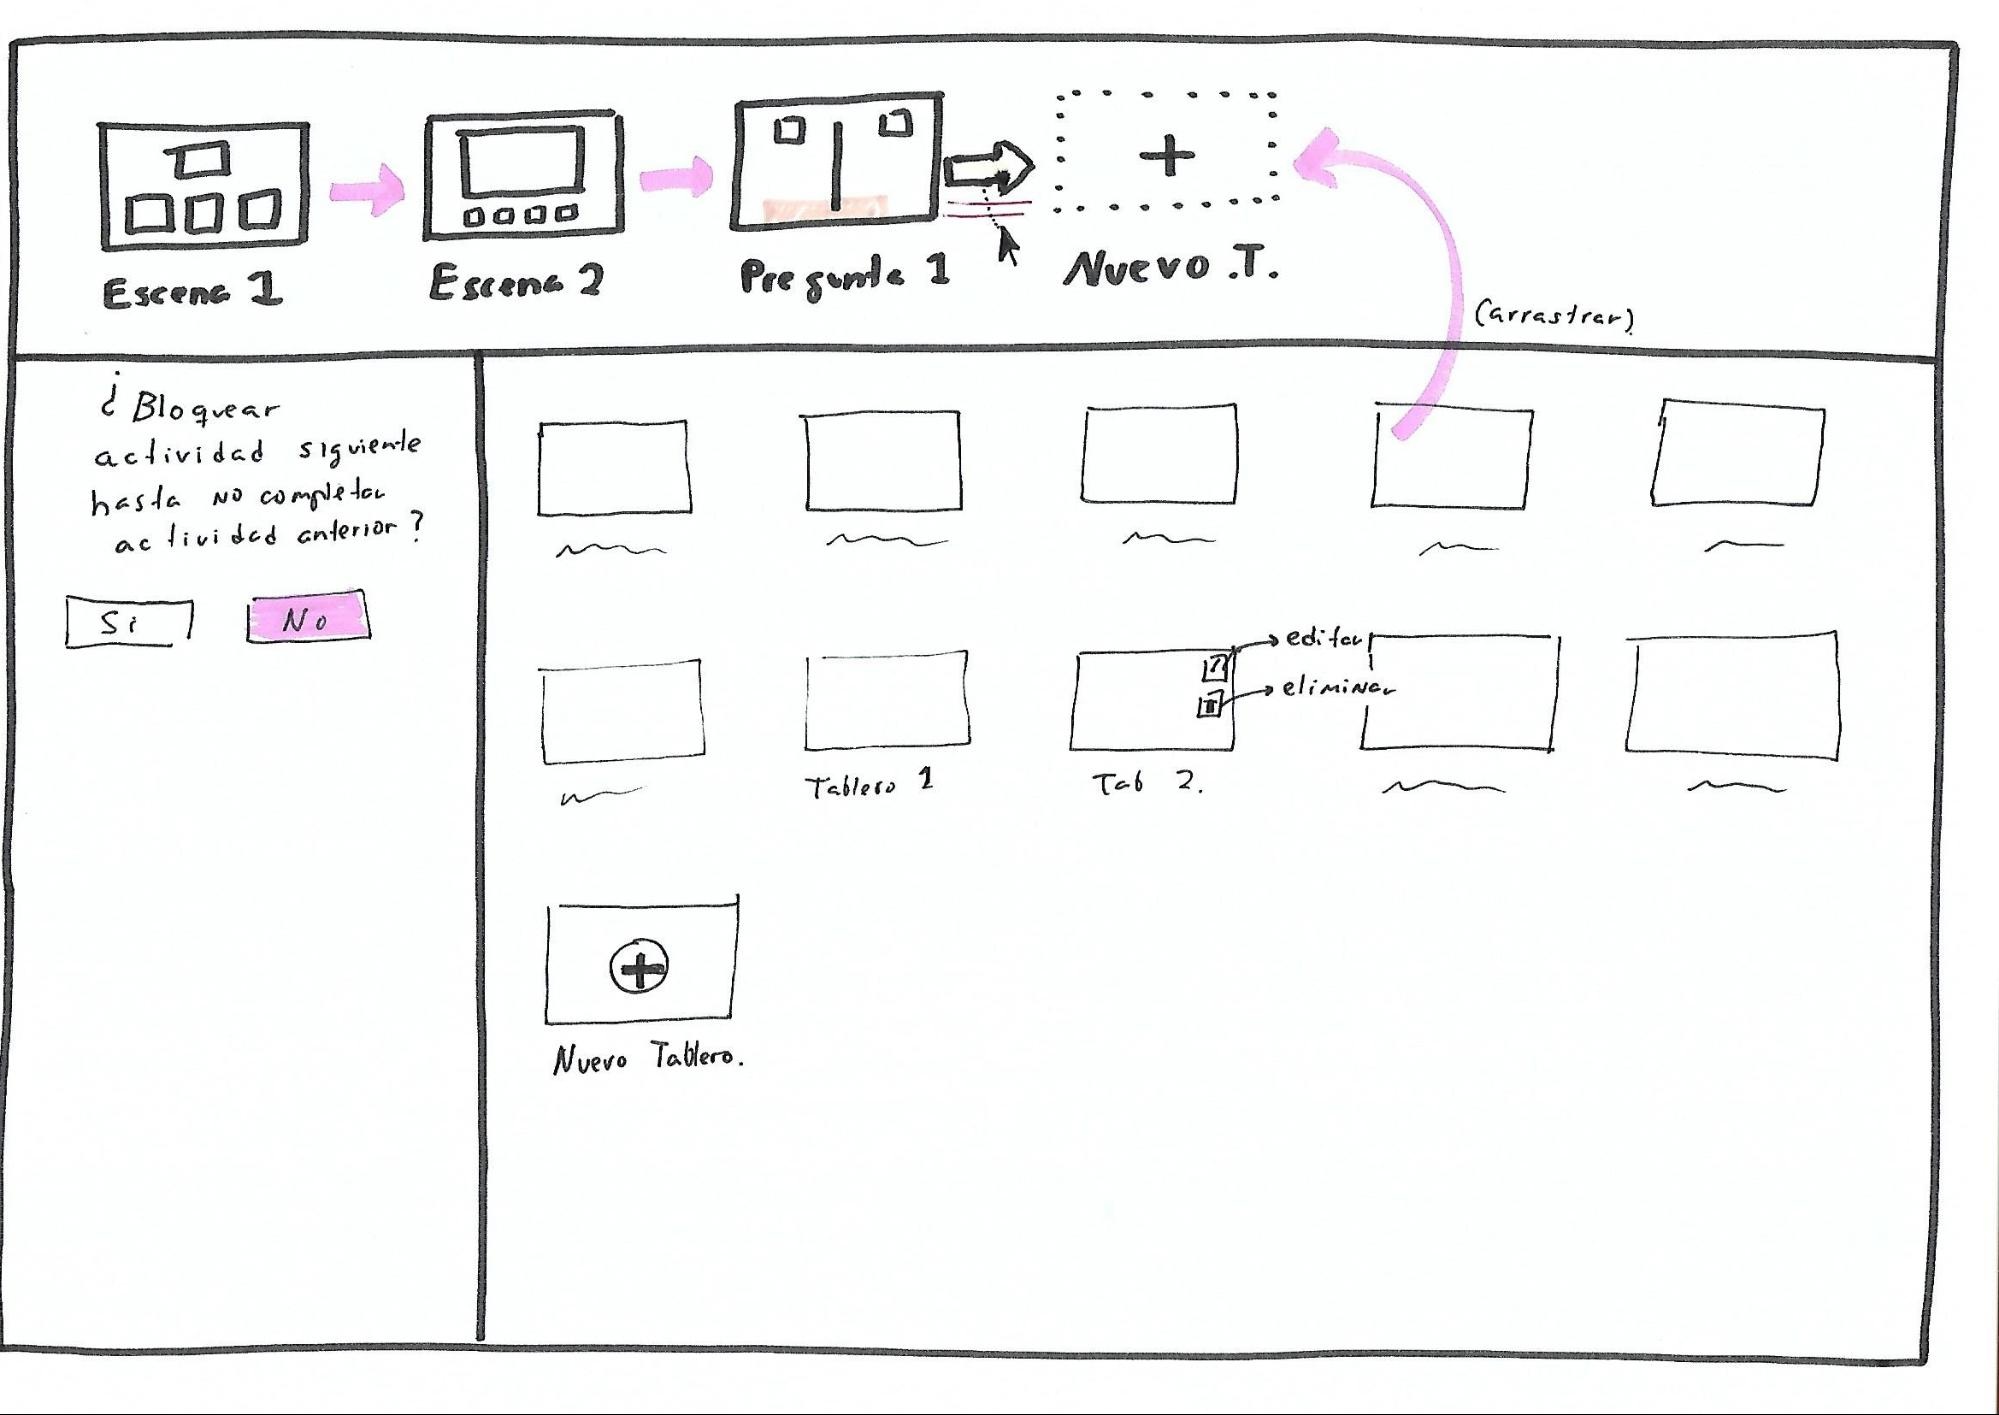
\includegraphics[width=0.7\linewidth]{Imagenes/Bitmap/presentacionTableros}
	\caption{Boceto del compositor de actividades}
	\label{fig:presentaciontableros}
\end{figure}


\subsection{Prototipo realizado por Jorge}
\label{cap4:sec:prototipo}
	
	La pantalla de inicio de la aplicación (ver la Figura \ref{fig:iniciojorge}) está compuesta por cuatro botones. Cada uno de ellos representará una pantalla con distintas funcionalidades. Tambíen podemos ver que en la parte superior de la pantalla tendríamos el nombre de la aplicación a la izquierda, que al pulsarlo volveríamos a esta pantalla, y un selector de idioma en la parte de la derecha. Esta parte sería común en las distintas pantallas de la aplicación.
	
	
% TODO: \usepackage{graphicx} required
\begin{figure}[h!]
	\centering
	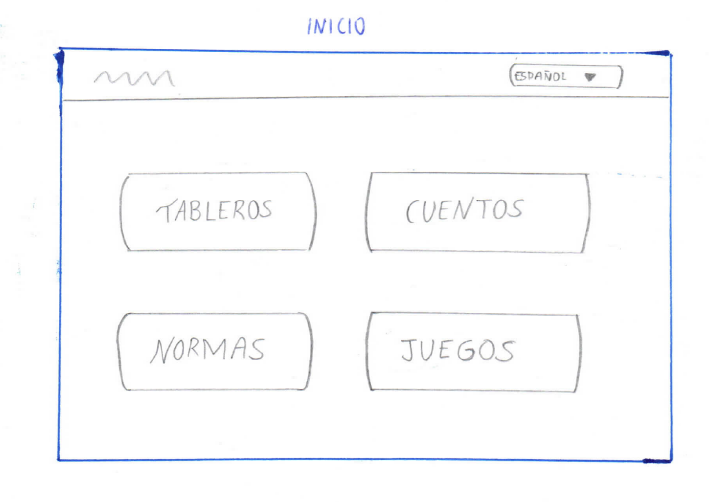
\includegraphics[width=0.7\linewidth]{Imagenes/Bitmap/inicioJorge}
	\caption{Pantalla de inicio con botones que muestran las otras pantallas de la aplicación.}
	\label{fig:iniciojorge}
\end{figure}

	
	En el apartado correspondiente a tableros representado en la Figura \ref{fig:tablerosjorge} podemos diferenciar claramente dos zonas: la parte de la izquierda correspondiente a la personalización del tablero y la parte de la derecha donde se mostraría el tablero que se está editando.
	
	
	En la parte de personalización del tablero podemos ver dos recuadros que englobarían diferentes posibilidades. Las funcionalidades que encontraríamos en el recuadro superior serían las siguientes:
	
	\begin{itemize}
		\item \textbf{Traducir frase}: dada una frase, mostraría toda la secuencia de pictogramas que tuviera ese significado. El botón de insertar que vemos insertaría toda la secuencia de pictogramas en el tablero.
		
		\item \textbf{Búsqueda simple de un pictograma}: dada una palabra concreta mostraría todos los pictogramas que tuvieran ese significado. Al igual que en el apartado anterior también tendríamos un botón de insertar el pictograma deseado al tablero.
	
	\end{itemize}

En el recuadro inferior tendríamos las siguientes opciones:

	\begin{itemize}
	
		\item \textbf{Insertar iconos}: al pulsarlo mostraría un modal con todos los iconos que se pueden añadir al tablero y al pulsar sobre uno de ellos se añadiría al tablero.
		
		\item \textbf{Insertar figuras geométricas}: al igual que con la funcionalidad anterior, al pulsarlo se abriría un modal donde se podrían seleccionar diferentes figuras geométricas para añadirlas al tablero.
		
		\item \textbf{Insertar imágenes}: esta herramienta permitiría al usuario insertar una fotografía que tuviera en su ordenador. A la hora de insertarla en el tablero tendrá las mismas propiedades que un pictograma, la imagen y un texto descriptivo.
		
		\item \textbf{Insertar un campo de texto}: permite añadir un campo en el tablero donde poner textos.
		
		\item \textbf{Editar el tamaño de letra del campo de texto}: esta funcionalidad solo estará disponible si hemos seleccionado un campo de texto en el tablero. Nos permite ajustar el tamaño del texto de un campo específico.
		
		\item \textbf{Editar la fuente del campo de texto}: al igual que con la funcionalidad anterior, deberemos seleccionar qué campo queremos editar. Permite cambiar la fuente del texto por otra.
		
	\end{itemize}
	
	
	En la zona inferior izquierda hay dos botones que permitirían guardar el estado de la página y volver a cargar el estado para posteriormente seguir trabajando con nuestro proyecto.
	
	
	En la zona de la derecha encontramos un tablero donde se insertaría todos los pictogramas, iconos, formas, imágenes y campos de texto. Todos los elementos que se inserten en el tablero podrán ser ampliados de tamaño pulsando sobre una de las esquinas del elemento.
	
	En la parte superior del tablero en sí tendríamos un botón llamado “\textit{Guardar como pdf}” que generaría un archivo con extensión pdf a partir del tablero inferior.
	
	Debajo de dicho tablero encontramos un botón que nos permitiría añadir un nuevo tablero con el que seguir trabajando.
	
	
	
	% TODO: \usepackage{graphicx} required
	\begin{figure}[h!]
		\centering
		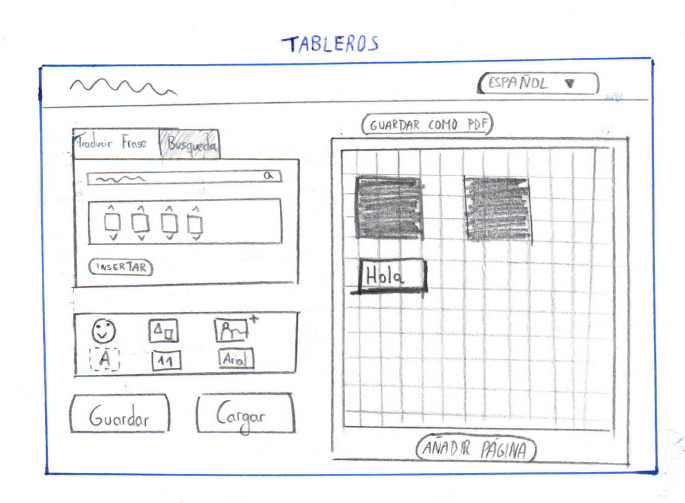
\includegraphics[width=0.7\linewidth]{Imagenes/Bitmap/tablerosJorge}
		\caption{Pantalla de configuración de tablero.}
		\label{fig:tablerosjorge}
	\end{figure}
	
	
	

	Respecto a las pantallas de normas y juegos son relativamente similares, ya que ambas en la parte de la izquierda cuentan con un apartado para la edición y a la derecha el tablero. Las únicas diferencias entre estas pantallas serían los botones que encontramos en el tablero para añadir una nueva norma o sección al cuento. Un ejemplo de la visualización de la pantalla de normas sería la Figura \ref{fig:normasjorge}. Ambas tienen un botón en la parte superior que ofrece la posibilidad de guardar como pdf lo que tenemos en el tablero.
	
	% TODO: \usepackage{graphicx} required
	\begin{figure}[h!]
		\centering
		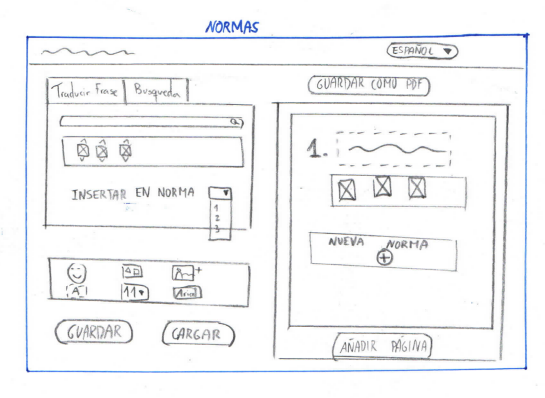
\includegraphics[width=0.7\linewidth]{Imagenes/Bitmap/normasJorge}
		\caption{Pantalla de configuración de normas.}
		\label{fig:normasjorge}
	\end{figure}


	
	Para añadir una norma o una nueva sección en nuestro tablero tendríamos que pulsar sobre el botón “\textit{Nueva norma}” o “\textit{Nueva sección}” y se añadirían dos campos. El primero de ellos estaría numerado y en él se insertaría el texto correspondiente a la norma o a la sección del cuento. El segundo sería un campo en donde poder insertar los pictogramas que queramos que hicieran alusión al campo de texto superior. Además, hay un botón para añadir un nuevo tablero y seguir trabajando.
	

	
	Por último la pantalla de juegos estaría compuesta por dos partes: la primera de ellas sería la configuración del juego y la segunda la ejecución del juego. La pantalla de configuración (ver la Figura \ref{fig:juegosjorge}), al igual que las pantallas vistas anteriormente, cuenta con una sección para la edición y otra para el tablero. En el tablero podremos ver las diferentes secciones que hayamos podido crear y un botón para crear una nueva. Al pulsar sobre este botón se añadirá sobre el tablero una casilla para insertar un pictograma, imagen, icono o figura geométrica, una flecha y un campo de texto. Esto permitirá crear una asociación entre un pictograma y su texto correspondiente para posteriormente ejecutar el juego.
	
	% TODO: \usepackage{graphicx} required
	\begin{figure}[h!]
		\centering
		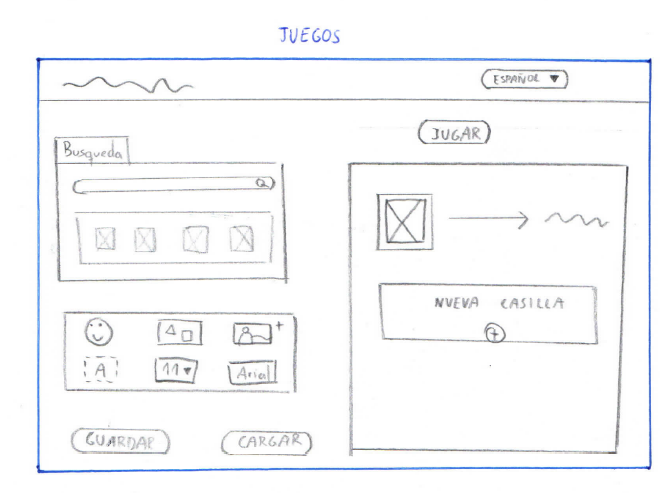
\includegraphics[width=0.7\linewidth]{Imagenes/Bitmap/juegosJorge}
		\caption{Pantalla de configuración de juego.}
		\label{fig:juegosjorge}
	\end{figure}

	Esta pantalla cuenta con dos botones para guardar el estado de la configuración del juego y otro para cargar dicho estado y reanudar el trabajo realizado.
	
	Tras haber creado varias secciones o haber cargado una configuración de juego podremos ejecutar el juego pulsando el botón “Jugar” situado en parte superior de la pantalla. Al pulsarlo nos llevará a una nueva pantalla más simple como se puede ver la Figura \ref{fig:juegojorge}, donde el usuario podrá ver todos los pictogramas que se han seleccionado en la pantalla de configuración y los textos asociados a cada uno de ellos.
	
	Todos los pictogramas seleccionados aparecerán en el recuadro superior de la pantalla. Estos pictogramas se podrán seleccionar y arrastrar a la casilla correspondiente de dicho pictograma. Si al arrastrar un pictograma y soltarlo en una casilla coincide con la norma definida por el usuario, la fecha que une la casilla del pictograma y el texto se pondrá en verde indicando que es correcta esa relación. En caso de que no corresponda el pictograma con el texto, el pictograma volverá a la parte superior donde se encuentran todos los pictogramas, indicando de esta manera que la asociación entre el pictograma y el texto no es la correcta
	 
	

	\begin{figure}[h!]
	\centering
	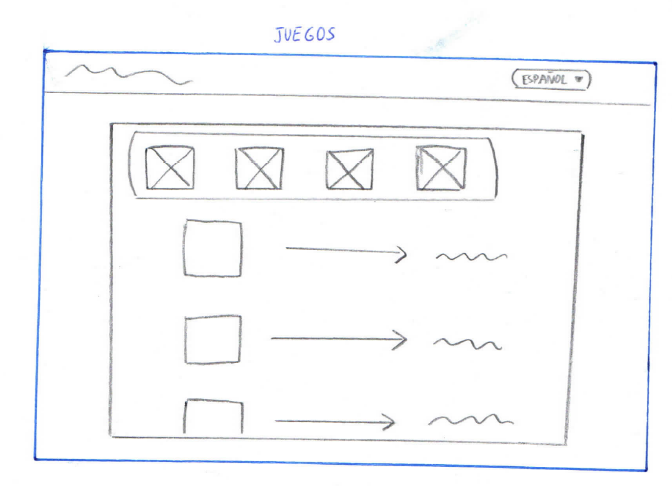
\includegraphics[width=0.7\linewidth]{Imagenes/Bitmap/juegoJorge}
	\caption{Pantalla de juego en ejecución.}
	\label{fig:juegojorge}
	\end{figure}
	

\section{Requisitos de la aplicación}
\label{cap4:requisitosapp}

Tras terminar ambos prototipos, se analizaron para contrastar ideas en común y estudiar posibles funcionalidades y elementos a implementar.

A grandes rasgos, se vio que el prototipo de Alfonso era menos rígido de cara a crear material. Esto es visible en la creación de reglas, cuento o actividades en el prototipo de Jorge, donde solo hay un único formato para cada tipo de material. Por ello se ha optado por ofrecer los componentes al usuario para que este cree el material según su criterio. Los componentes de creación de actividades vistas en el prototipo de Alfonso también ofrecían mayor libertad al crear actividades. 

Un concepto en común entre ambos prototipos es la existencia de una barra de herramientas al lado izquierdo del tablero mediante la cual se añadirían los distintos elementos al tablero. Además, se estableció que debían existir dos tipos de componentes en la aplicación: herramientas y elementos.
A continuación se detallarán las funcionalidades que deberían desempeñar estas componentes. El resto de ideas vistas en ambos prototipos sirvieron para crear una visión general de la posible aplicación, por lo que muchas de estas ideas no fueron desarrolladas.  

\subsection{Herramientas}

En este apartado se incluirán todas aquellas funcionalidades que tras el análisis fueron determinadas como necesarias para desarrollo de la aplicación. Principalmente estas funcionalidades estarán relacionadas con la edición del tablero. Las funcionalidades que se decidió desarrollar fueron:

\begin{itemize}
	\item \textbf{Búsqueda de pictogramas}: esta herramienta permitirá al usuario realizar una búsqueda a partir de una palabra y poder añadir al tablero el pictograma deseado.
	
	\item \textbf{Traducción de frase}: esta herramienta permitirá generar una secuencia de pictogramas asociados a una frase introducida por el usuario y poder añadir esa secuencia al tablero.
	
	\item \textbf{Colecciones}: la herramienta colecciones ofrecen al usuario la opción de poder tener varias agrupaciones de los pictogramas que desee, según su conveniencia. Éstas están compuestas por un nombre que lo identifique y uno o varios pictogramas que el usuario elija según su criterio.
	
	\item \textbf{Importar imágenes}: esta herramienta permite al usuario importar sus imágenes y fotografías y añadirlas al tablero. 
	
	\item \textbf{Añadir texto}: la herramienta de texto permitirá añadir una frase introducida por el usuario al tablero. 
	
	\item \textbf{Añadir icono}: esta herramienta permite añadir al tablero iconos para complementar a los pictogramas, textos o imágenes.
	
	\item \textbf{Importar y exportar}: estas herramientas ayudarán al usuario a poder guardar el estado de la página y poder editarlo posteriormente. 
	
	
\end{itemize}

\subsection{Elementos}


En esta sección analizaremos los principales componentes que se podrán usar en los tableros, como paso previo a su implementación.

Hemos considerado que un elemento es un componente que puede ser añadido al tablero. Distinguiremos dos tipos de componentes: los básicos que no añaden ninguna interacción, y los componentes interactivos. Estos pueden ser ajustados y añadir comportamientos específicos para el usuario que utilice el tablero creado.

\begin{itemize}
	
	
	\item \textbf{Picto}: el elemento picto representa un pictograma junto a su nombre asociado. Cuenta con la opción de poder modificar algunas características del pictograma, como indicar un tiempo verbal. Si el pictograma muestra a una persona, también se puede cambiar el color de pelo y tono de piel.
	
	\item \textbf{Foto}: el elemento foto permite añadir imágenes tanto a partir de una URL como las que suba el propio usuario. Esta ha sido una de las características más demandadas por los usuarios. El permitir añadir fotos abre multitud de posibilidades, como la de poner fotos de la familia, mostrar localizaciones habituales como la cocina e identificar objetos personales que no se representan tan fielmente mediante un pictograma (por ejemplo un juguete específico o la portada de su  libro favorito). Esto facilita al usuario final relacionar conceptos al mostrar figuras que le sean familiares.
	
	\item \textbf{Figuras}: las figuras sirven para ordenar, enfatizar o decorar el tablero. Por ejemplo,  una línea puede ser usada para dividir el espacio de trabajo en secciones, relacionar dos pictogramas o incluso marcar un espacio donde escribir una respuesta si se va a imprimir el tablero. Pese a la simplicidad de las figuras, sus posibilidades son muy amplias según  la creatividad de quien crea el tablero.
	
	\item \textbf{Campos de texto}: Los campos de texto podrán ser insertados en el tablero de la aplicación. Estos campos de texto podrán ser editados permitiendo cambiar el color del texto y aumentar la fuente.
		
\end{itemize}

Hay algunos elementos que tras el análisis de los prototipos decidimos que no iban a aportar lo suficiente en la aplicación o que incrementarían innecesariamente la complejidad. Estos elementos descartados fueron:

\begin{itemize}
	\item\textbf{Pantallas de normas y cuentos predefinidos}: El principal motivo es su falta de flexibilidad, es decir, que si la aplicación no permite crear un cuento o un listado de reglas con sus propias herramientas, tampoco permitirá crear otro tipo de material. Por ello nos hemos decantado por herramientas que ofrecieran más posibilidades al usuario. Otro motivo era que no todos los usuarios querrían por ejemplo que las normas aparecen de una misma manera, como si fuese un listado, por lo que es imprescindible ofrecer la mayor libertad posible al usuario.
	
		
	\item \textbf{Cajón de pictogramas}: El cajón de pictos es un apartado al margen del tablero donde aparecen un conjunto de pictogramas que el usuario debe mover a alguna posición. El hueco donde vayan los pictogramas que se encuentren en el cajón de pictogramas puede ser modificado y aceptar unos u otros. Esto puede ser utilizado como test sencillo de hacer y usar.
	
	\item \textbf{Subtablero}: El subtablero es un componente que a simple vista parece un pictograma pero, al ser pulsado, despliega un tablero que contiene otros pictogramas. Este concepto es originario de Piktoplus pero actualmente no cuenta con soporte y puede ser de utilidad para añadir más pictogramas en el mismo espacio.
	
	\item \textbf{Plantillas}: Tras comentarlo en las reuniones, no se centró mucha atención en este apartado, pues ya estaba muy explorado por la aplicación Pictableros (Sección \ref{cap2:pictableros}).
	
	\item \textbf{Log In}: El principal motivo de su descarte fue el no poder garantizar en un primer momento la total seguridad de los tableros creados.
	Otra de las características del proyecto es la inclusión de imágenes que pudiera subir el usuario, con la responsabilidad añadida de estar manejando imágenes de menores de edad. Estos fueron los motivos por los que optamos por una modalidad sin necesidad de servidor, donde los documentos generados se guardan en el ordenador.
	
	\item \textbf{Selección de idioma}: Fue una idea descartada al principio del desarrollo, en vista de que la gran mayoría de las aplicaciones existentes ofrecían soporte en multitud de idiomas. Pero no se llevó a cabo para centrarnos en otros aspectos de mayor relevancia en el contexto del trabajo.
	
\end{itemize}


\section{Reglas de diseño}
\label{cap4:sec:reglas}
Para asegurar un correcto desarrollo de las distintas funcionalidades que se encuentren en la aplicación, se tendrá en cuenta las ocho reglas de oro de Ben Shneiderman\footnote{\url{https://www.interaction-design.org/literature/article/shneiderman-s-eight-golden-rules-will-help-you-design-better-interfaces}}. A continuación serán enumeradas: 


\begin{itemize}
	
	\item \textbf{Coherencia}: se ha de utilizar los mismos tipos de patrones de diseños en toda la aplicación. Esto incluye los colores, el tipo de letra utilizado, la posición de los botones, etc. Esta regla es de vital importancia ya que facilita al usuario familiarizarse con la interfaz.
	
	\item \textbf{Usabilidad universal}: ha de tenerse en cuenta que la aplicación la pueden utilizar distintos tipos de usuario. A los usuarios más avanzados se les ha de dar la oportunidad de utilizar funciones más complejas frente a los usuarios principiantes. 
	
	\item \textbf{Retroalimentación} informativa: se ha de informar a los usuarios en todo momento de las acciones realizadas de manera visual, por ejemplo mediante cuadros de diálogo.
	
	\item \textbf{Diseñar diálogos para conducir la finalización}: las acciones que requieran de unas ciertas secuencias deberán estar bien organizadas para informar al usuario sobre el momento del proceso en el que se encuentra.  Es importante que tengan una etapa de comienzo, otra de desarrollo y por último una de finalización.
	\item \textbf{Prevenir errores}: se ha de diseñar la interfaz de la aplicación de tal manera que los usuarios cometan el menor número de errores posible. Un ejemplo recurrente es deshabilitar botones o menús. En caso de que ocurra un error se deberá informar al usuario indicando el fallo y las posibles soluciones. 
	
	\item \textbf{Permitir deshacer acciones de forma fácil}: todas las acciones que se realicen en la aplicación deben de ser reversibles. Esto permite a los usuarios realizar acciones sin temor a no poder revertir los cambios realizados.
	
	\item \textbf{Maximizar la sensación de control}:  las acciones no deberían de superar los tres clics. No hay problema si el número es superior siempre y cuando el usuario sepa en todo momento las acciones que está realizando. 
	
	\item \textbf{Reducir la carga de memoria a corto plazo}: es importante que la información que se muestre al usuario sea breve y concisa. Además también es importante agrupar todas aquellas funcionalidades similares para reducir la carga de memoria del usuario.
	
\end{itemize}


